% !TeX spellcheck = en_US
\documentclass[10pt,a4paper,twocolumn,twoside]{article}
\usepackage[utf8]{inputenc}
\usepackage[english]{babel}
\usepackage{multicol}
\usepackage{graphicx}
\usepackage{fancyhdr}
\usepackage{times}
\usepackage{titlesec}
\usepackage{multirow}
\usepackage{lettrine}
\usepackage{pdflscape}
\usepackage{subcaption}
\usepackage{booktabs}
\usepackage[edges]{forest}
\usepackage{url}
\usepackage[top=2cm, bottom=1.5cm, left=2cm, right=2cm]{geometry}
\usepackage[figurename=Fig.,tablename=Table]{caption}


\author{\LARGE\sffamily Segovia Barreales, Richard}
\title{\Huge{\sffamily Reducing dizziness when using a video-see-through head-mounted display}}
\date{}

\newcommand\blfootnote[1]{%
	\begingroup
	\renewcommand\thefootnote{}\footnote{#1}%
	\addtocounter{footnote}{-1}%
	\endgroup
}

%
%\large\bfseries\sffamily
\titleformat{\section}
{\large\sffamily\scshape\bfseries}
{\textbf{\thesection}}{1em}{}

\begin{document}
	
	\fancyhead[LO]{\scriptsize AUTHOR: SEGOVIA BARREALES, RICHARD}
	\fancyhead[RO]{\thepage}
	\fancyhead[LE]{\thepage}
	\fancyhead[RE]{\scriptsize EE/UAB TFG INFORMÀTICA: REDUCING DIZZINESS WHEN USING A VIDEO-SEE-THROUGH HEAD-MOUNTED DISPLAY}
	
	\fancyfoot[CO,CE]{}
	
	\fancypagestyle{primerapagina}
	{
		\fancyhf{}
		\fancyhead[L]{\scriptsize TFG EN ENGINYERIA INFORMÀTICA, ESCOLA D'ENGINYERIA (EE), UNIVERSITAT AUTÒNOMA DE BARCELONA (UAB)}
		\fancyfoot[C]{\scriptsize May 2018, Escola d'Enginyeria (UAB)}
	}
	
	\renewcommand{\headrulewidth}{0pt}
	\renewcommand{\footrulewidth}{0pt}
	\pagestyle{fancy}
	
	\maketitle
	
	\thispagestyle{primerapagina}
	
	
	\blfootnote{$\bullet$ E-mail: richard.segovia@e-campus.uab.cat}
	\blfootnote{$\bullet$ Menció en Computació}
	\blfootnote{$\bullet$ Project supervised by: Coen Antens (CVC) and Felipe Lumbreras (Computació)}
	\blfootnote{$\bullet$ Course 2017/18}
	
	\section{Introduction}
	
	\lettrine[lines=3]{T}{his} project has its origins in the internship that I done in the Computer Vision Center (CVC) in summer 2017. During my internship I developed a basic video-see-through viewer for a head mounted display (HMD) developed in the CVC. Along with the development we discovered that the main concern that our prototypes faced during our user testing sessions was the feeling of dizziness and motion sickness produced by the headset. Hence the motivation for this project, reduce the adverse physical reactions that it produces to the users \cite{disconfortReview}, \cite{unpublishCVC} and continue improving the viewer making adding new modules while keeping its expandability. It has to be said that this research project is focused mainly on the software, the prototypes and other hardware aspects will be out of our concerns and will be developed by CVC researchers. A communication channel though is opened to discuss about the development of the whole project. 
	
	The head mounted displays first appeared in 1965 when Ivan Sutherland developed the first HMD called "the sword of Damocles" \cite{hdmSutherland}, it stablishes the ground for further development in the field. The development of these technologies has grown in the last years mainly centered in the video-games field. Some examples, are the Oculus \cite{web:oculus} or the HTC Vive \cite{web:vive}. These products are virtual reality headsets, therefore they are only capable of showing computer generated scenes. The developed project prototypes differ in this matter because they can also show the real world, this kind of HMDs are called video-see-through, the current version of the prototype can be seen in Figure \ref{fig:proto}.
	
	%si contemplamos el estado actual del mundillo, en general, las aproximaciones a variaciones en la vergencia se hacen apartir de la visualizacion del comportamiento del ojo, posicion para poder calcular la vergencia 
	
	
	\section{Objectives}
	
	\subsection{Initial objetives}
	First, we will be developing a software that will be capable of capture stream from a stereo camera and display it in real time. The software will show one camera stream on each half of the screen, also the HMD will enable only to each eye to see one half of the screen, all of this will simulate the stereo effect (creating a depth effect). Another goal is to prepare this software to be easily expandable with new modules in the future.
	
	Second, as is reported in \cite{disconfortReview}, and we discovered in a user testing session in the CVC \cite{unpublishCVC}, using head mounted displays can cause a variety of adverse physical reactions, since this HMD will be used while working, these symptoms will reduce the concentration and the effective working hours. For that reason, reducing these adverse physical reactions is a priority. To achieve this goal, we will try to apply two techniques: 
	
	\begin{figure}
		\centering
		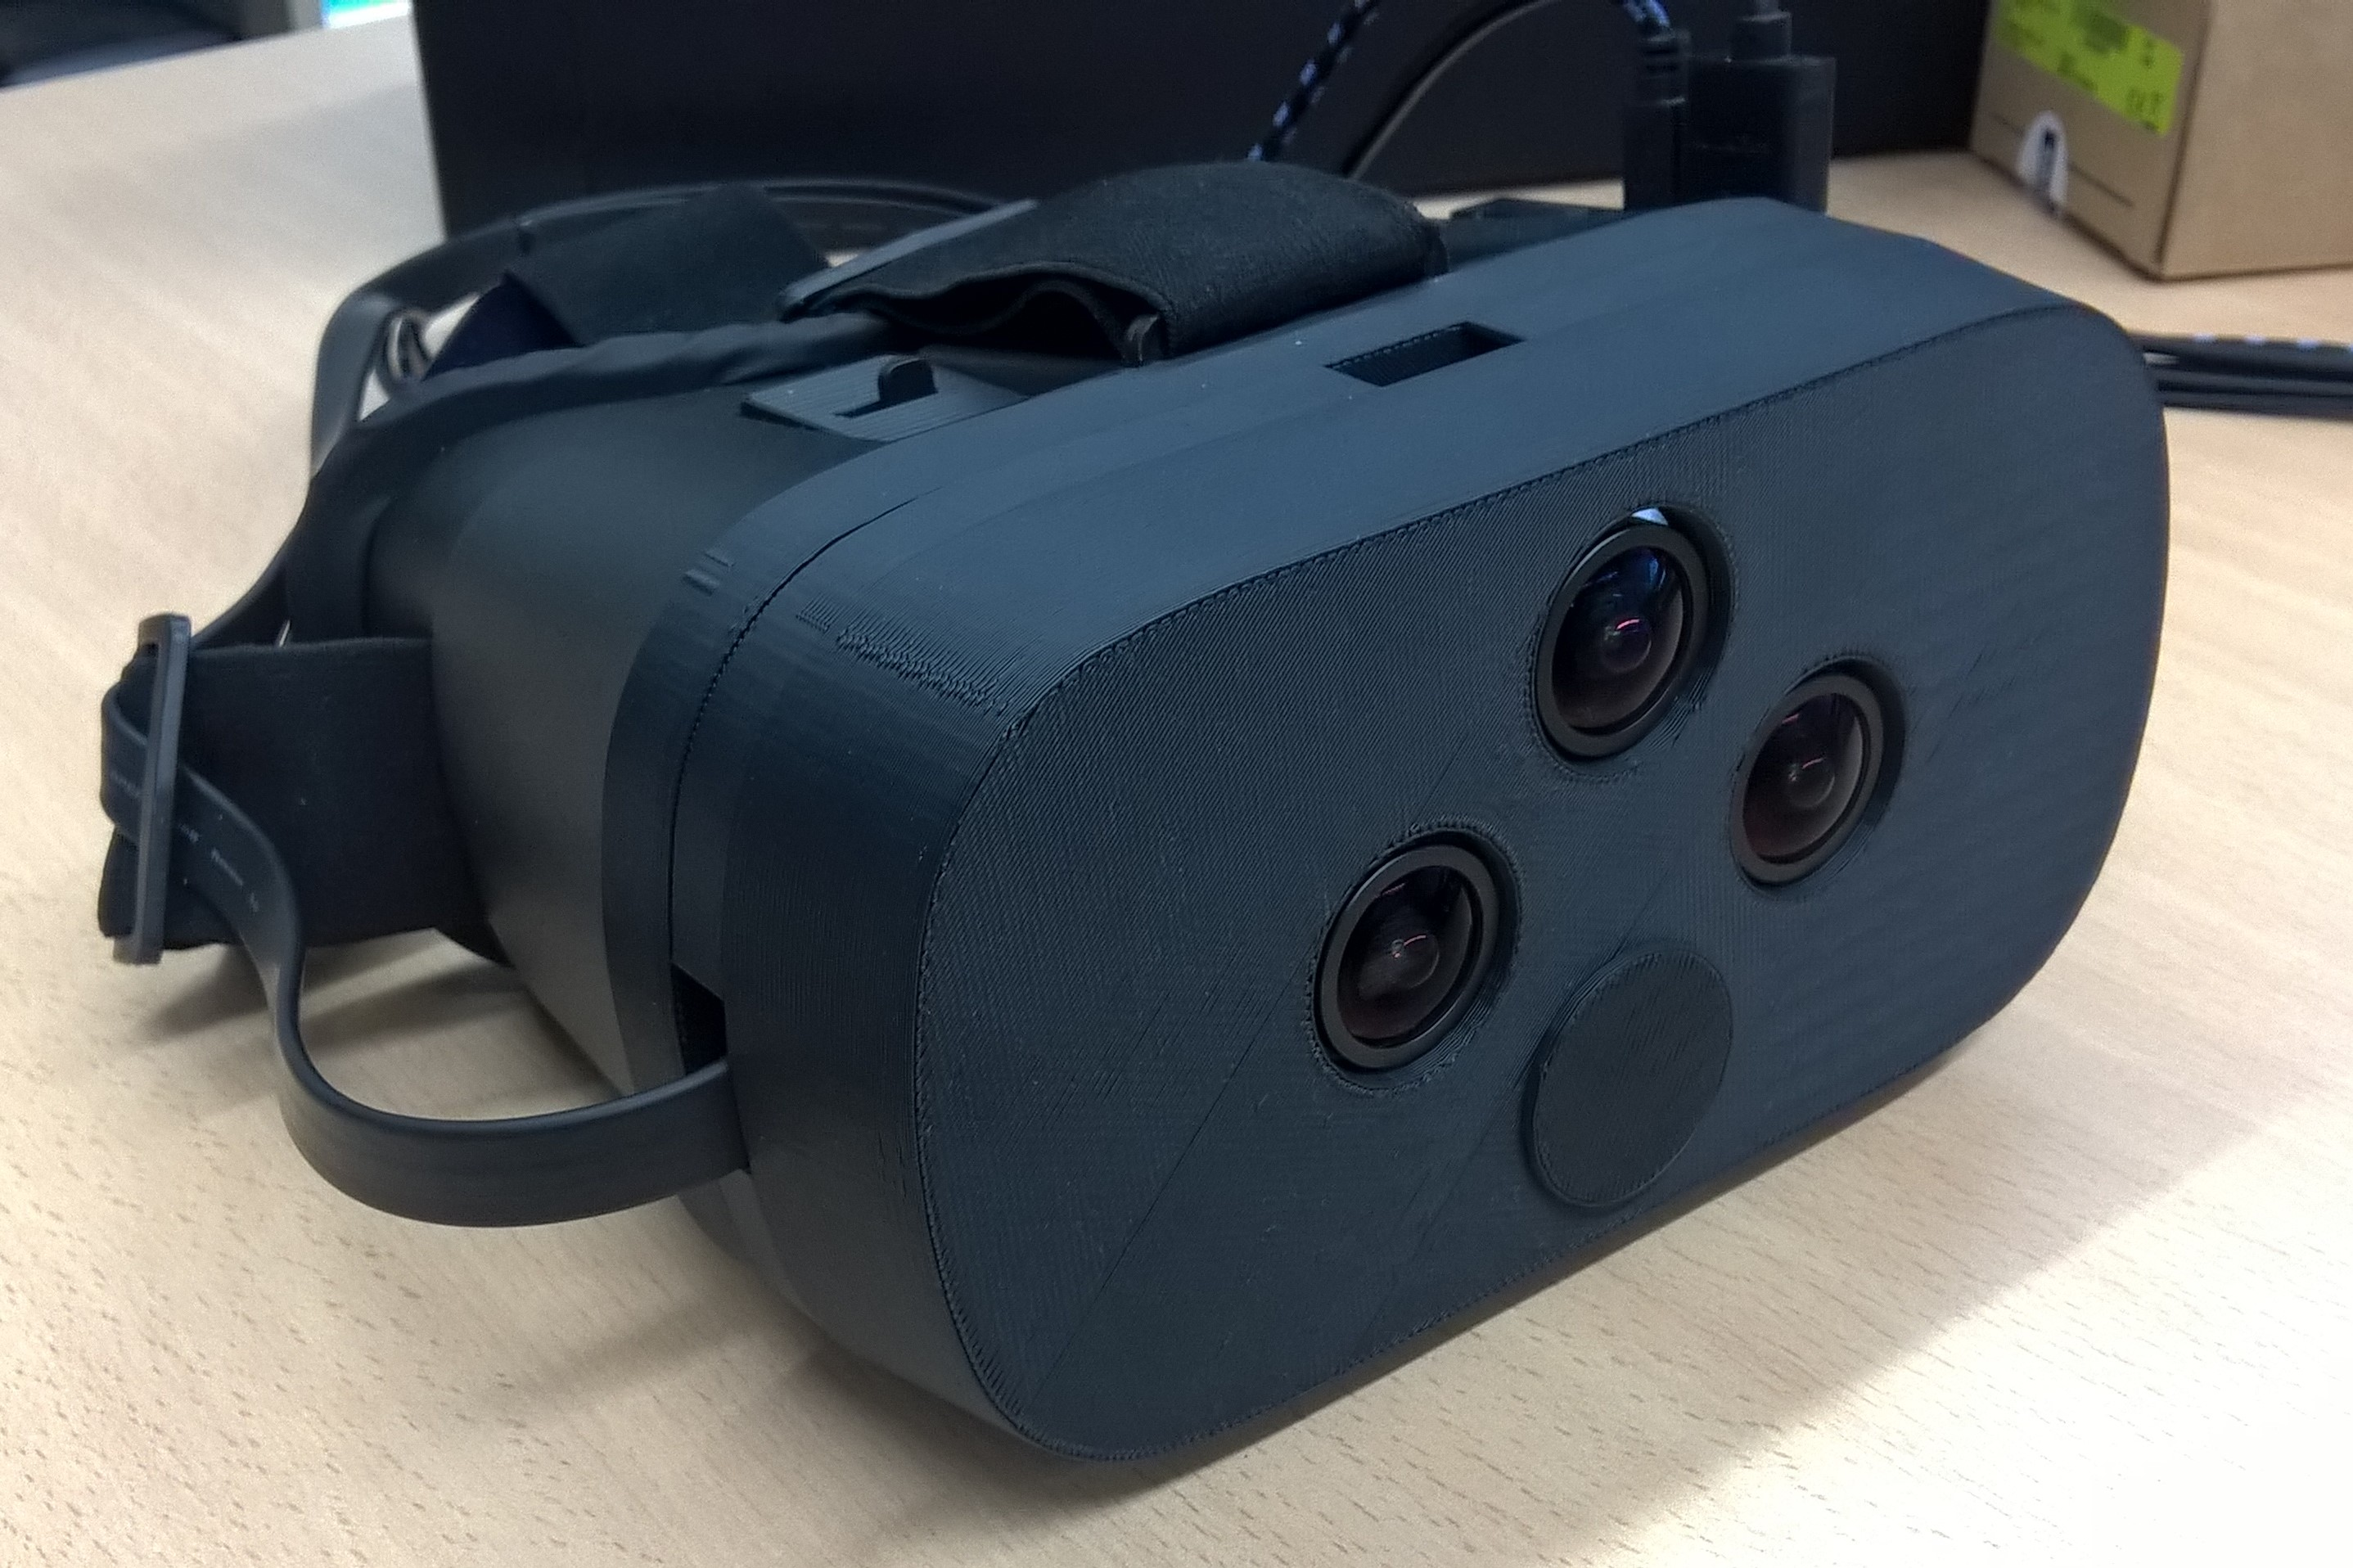
\includegraphics[width=1\linewidth]{img/imagenproto3.jpg}
		\caption{Current version of the HMD video-see-through prototype.}
		\label{fig:proto}
	\end{figure}
	
	\begin{itemize}
		\item Accommodation-Vergence: As is reported in the \cite{disconfortReview}, \cite{vergenceDisconfort} articles the mismatch between accommodation and vergence in head mounted displays causes a conflict on the expected depths increasing the feeling of discomfort and dizziness.  One idea to reduce this effect is to dynamically move the position of screen frames as the focus changes from closer to distant objects and vice versa. To achieve this, we will use a neural network that will be able to discern between closer and distant objects, also we will need the depth map obtained via the stereo camera setup. \\*
		In addition, a progressive change from one focus to the other may be needed, as a big change in focus can induce sickness to the user.
		
		\item Depth of field (DoF) blur: Recent investigations \cite{ifftConfortDoF} suggest that applying a DoF blur to a scene viewed using a head-mounted display can reduce visual discomfort, the challenge here is that our project has to make this DoF blur in real time in a real world environment, in contrast to the developed in that investigation where they used computer generated scenes. To achieve this, we are going to use disparity map and the information obtained by a neural network that discerns between closer and distant objects.
	\end{itemize} 
	
	Third, as the HMD will be used in workplaces, the idea of adding data to the environment, could improve the work-flow and the work efficiency. For this reason, we think, that adding a third camera to the system can add valuable information that can be mixed with the environment. A similar idea can be found here \cite{vismerge} where a third camera is used to add information to the real world. For example, by adding an infrared camera, the user can be warned by highlighting objects too hot to be touched.
	
	Fourth, as we discovered in a user testing done in the CVC \cite{unpublishCVC} last January, using a computer while wearing the HMD is a difficult task, mainly because the screen was unreadable for the brightness saturation of the image. For that reason, a system capable of detecting computer screens and adapt the brightness, contrast and others parameters of the image stream will be developed.
	
	Along all the development, user testing sessions will take place to check the improvements made between the different versions of the developed software and the different prototypes developed. The main goal of this sessions will be to evaluate whether the developed software works and if it reduces the sickness feelings of the users. The procedure used in the user testing will be like the performed in \cite{ifftConfortDoF}, where the Simulator Sickness Questionnaire \cite{ssqQuestion} where used to evaluate the symptoms. 
	
	\subsection{Progress and changes}
	
	After these firsts weeks of development some objectives have changed and other have appeared, as we will explain in section \ref{sec:planning}, the main issue was that the depth map generation needed some work before integrating it into the system.
	
	The integration of a reliable depth map generation is essential to the project, it is needed to complete both Accommodation-Vergence and DoF goals, and as it give us knowledge of the environment it would probably be key in future developments. For these reasons it was decided to add it as an objective itself. The main goal will be to integrate a fast and reliable depth map generator with all the required components.
	
	As the depth map generation requires a stereo pair of undistorted images to obtain a reliable depth map, the integration of a system capable of read calibration files or calibrate itself and undistort the output of the cameras is required.  

	The performance of the depth map generation is also a key issue, as a slow image generation will give the system great latency and that could limit the uses cases of the module. 
	
	The current objectives and tasks list can be found in the appendix, it was done to recollect all the goals that this project want to achieve. Future references to the objectives and tasks will use the appendix list numeration. As we will see in \ref{sec:planning}, not all of this goals will be reachable due to time constraints.
	
	\section{Methodology}
	Scrum and its variants are one of the most spread work methodologies nowadays.
	The Scrum methodology is the selected to be used in this project, however, as this project will only be done by one person, some changes have to be made. 
	
	First as there is only one developer the daily meeting will be substituted with a weekly meeting with the stakeholders, in this case the tutor and the boss of the laboratory department in the CVC, in these meetings we will evaluate the development done, the issues faced that week and the problems solved. In addition to that we will discuss and review future milestones and the progress towards them.
	
	Second, a backlog will be prepared at the beginning of the project and will contain the main goals divided in tasks, these tasks will be organized in groups of sprints easily done in a week. As each sprint has a backlog of task to be done, a tool can be used to organize this backlog, in this case Trello\cite{web:trello} will be used.
	
	Third, each iteration over the documentation and the development will be kept by a version tracker, in this case, Github \cite{web:github} and its desktop client \cite{web:githubDesktop}. 
	
	Keeping the main scrum methodology, I think it is interesting to grab some ideas from the Lean software development \cite{web:leanMethod}. The idea of removing the so called "Muda", non-important extra features and processes, could be beneficial for this project because it could reach an overwhelming dimension for the limited time that is had.
	
	Involving the tools that will need to be used develop the project, first of all, the current viewer version is made in C++ using the QT libraries \cite{web:qt}, therefore any tools that would be used need to be compatible with the current version of the viewer. For that reason among others, TensorFlow\cite{web:tensor} was chosen as the main library for building the neuronal network. Currently, tensor supports  Python and C++\footnote{Currently, the TensorFlow's C++ runtime is only available for Linux.}as development language. In addition to that it is also possible to save a trained model in tensor and load it using OpenCV both in Python and C++. Other reason to choose tensor over other alternatives is because is commonly used by the CVC researchers, therefore, if any advice is needed, it can be solved asking one CVC researcher.
	
	The custom scrum methodology already explained has been followed without any change in the development. Every part of the development process has been documented and every change in the code has been uploaded to a private Github repository. It is worth mention that the OpenCV \cite{web:opencv} library has been used to develop the calibration and undistort module. 
	
	Once the tasks \ref{obj:dispmap}, \ref{obj:acc:preset} and \ref{obj:acc:dispmap} were finished, a protocol was designed in order to do every user testing session in the same conditions. It has the following considerations: 

	\begin{itemize}
		\item To perform the testing, 3 ophthalmological patterns will be set in 3 different locations, one at reading distance, other at close distance, like the pc screen; and other far away at the wall of the room. 
		\item  Each user will do one session per day and the distance calibration done by the user will be done in a random order. 
		\item  Every user will rest for a few seconds between each calibration of the preset.  
		\item  Every preset calibration will start in with the camera images in the center of the ROI. 
		\item  Once the user calibration is finished, every user will comment its feelings when using a setting preset in the other distances. 
	\end{itemize}
	
	
	\section{Planning}
	\label{sec:planning}
	
	\subsection{Dataset}
	\label{subsec:dataset}
	To be able to develop this project a dataset will be necessary to train the neural networks and to check the depth map. In this case as we have available three hardware prototypes, a data collection procedure will be possible and simple. For that reason, a dataset caption session is planned.
	
	Also, a dataset will be used to make sure our dataset is correct and to encompass a broader range of environments. For that reason, we selected first the Middlebury stereo dataset \cite{web:middelburyDataset} because it has a great dataset of stereo images and the groundtruth of their depth map. Additionally a dataset with indoor and outdoor scenes is recommended. Several dataset could be used with that purpose, for example the MIT's places dataset \cite{web:mitplaces} and the INDSECS indoors only dataset \cite{web:indecs}.
	
	A calibration dataset is required to generate a quality calibration. This dataset will contain a series of images of a chess like pattern located in different parts and depths of the image. A requirement is that the patterns appears completely in both camera. This dataset will be updated every time the cameras or the HMD gets manipulated, this is because any minor change in the focal length or the position between the cameras will affect the results of the calibration.
	
	To be able to evaluate the depth map generation, a video sequence of the stereo pair must be captured and later processed by the depth map module. It would be convenient the integration of a video capture module to the current program to ease the evaluation task.
	
	%for the next report: a dataset with different scenarios were captured in order to test the potencial of the depth map and the libelas thingy
	
	\subsection{Accommodation-Vergence}
	\label{subsec:vergence}
	In this stage, a neural network will be trained to detect the distance of the focus and the necessary vergence in the screen placement to help the user a more comfortable experience.
	This will, alongside with the DoF blur, be the main time-consuming stage of the project and will have the following parts:
	\begin{enumerate}
		\item \label{itm:preset}  Preset creation: In this task, the current viewer will be expanded with the creation of multiple and easy to change presets that will allow further user testing.
		
		\item \label{itm:UserTesting} User testing, presets: In this first user testing session after the finalization of task \ref{itm:preset}, the users will be told to configure their own focus settings and to try to change between them to adapt the focus to closer or distant objects. The goal here is to acknowledge whether the user feels better accommodation with the focus between objects.
		
		\item \label{itm:ProgressivePreset} Progressive preset change: After the development of \ref{itm:preset} and \ref{itm:UserTesting}, if the users report sickness because of the sudden change between presets, a smooth transition between them will be developed to reduce the issue. 
		
		\item Disparity map: In parallel with the development of the tasks \ref{itm:preset}, \ref{itm:UserTesting} and \ref{itm:ProgressivePreset}, a disparity map generator from a stereo pair is required to continue with further development. As this subject is complex per se and is not the main goal of this project, a library that already implements a good stereo matcher, like LIBELAS\cite{web:LIBELAS}, will be used. 
		
		\item Neural network with camera streams: This task will start after the analysis of the data collected in the task \ref{itm:UserTesting}. The main goal will be to create a neural network capable of returning the value of the vergence. To achieve this several architectures will be tested and compared, with one, two or three streams from the cameras and including the disparity map information when developed.
		
		\item User testing: In this user session, the goal will be to check if the development done in this stage has reduced the sickness feelings of the users, and with which solution the user feel more comfortable.
	\end{enumerate}
	
	\subsection{Depth of field blur}
	This stage will be developed after the finishing of the previous Accommodation-Vergence phase \ref{subsec:vergence} and shares some development with it. 
	
	This problem can be resolved in to ways, using a disparity map only to create the DoF and using Neural network to aid the creation of it.
	
	\begin{enumerate}
		\item Mock up blur: to ensure that the results of \cite{ifftConfortDoF} are applicable to real world scenarios, a mock up blur photo dataset will be made, and a user testing session will take place.
		
		\item Designing de pipeline: this task goal is to design, both pipelines, the disparity map only and the neural network aided.
		
		\item \label{itm:disparityversion} Disparity map version: this version will generate the DoF blur using only the disparity map to obtain the depth and using the center point of the cameras as the focus point.
		
		\item \label{itm:NNversion} Neural network adaptation: this task will take the neural network developed in the previous phase and will modify it to make it usable in this phase of the project. The idea is that this network will produce an indicative value of the blurriness needed using the camera images to determine whether the scene has closer or distant objects.
		
		\item User testing: Along with the development of \ref{itm:disparityversion} and \ref{itm:NNversion}, a user testing session will take place to check whether this system has reduced the dizziness and which solution is more comfortable for the user.
	\end{enumerate}
	
	\subsection{Improving screen quality}
	In this stage a system to improve the quality when the user is looking a screen will be developed. This system can be split in two tasks:
	\begin{enumerate}
		\item \label{itm:QualityImprovements} Quality improvements: In this task a system capable of changing contrast, brightness and other image parameters will be developed, this system will not be automatic and will need the interaction of the user.
		
		\item Automatic switching: The goal of this task will be to free the user from the interaction with the system developed in task \ref{itm:QualityImprovements}, to achieve this a neural network will be developed to detect when a user is looking a screen.
	\end{enumerate}
	
	Part of the development of this objective will be left to future projects due to time constrains.
	
	\subsection{Third camera}
	This stage will have as a main goal the integration of a third camera in the viewer software and highlighting relevant information obtained using the third camera on stream viewed by the user. It can be split in the following tasks.
	
	\begin{enumerate}
		\item \label{itm:Integration} Integration with the viewer: Introducing a third camera in the system will mean making some modifications in part of the viewer code. The goal of this task will be to prepare the different modules of the viewer for the introduction of the third camera.
		
		\item Research mixture: After the development of task \ref{itm:Integration}, a system to allow the mixture of images between visible and the third camera spectrum will be developed, the goal will be to add information to the user from the third camera different spectrum.
	\end{enumerate}
	
	Part of the development of this objective will be left to future projects due to time constrains.
	
	
	\subsection{Research, documentation and planning}
	This stage of the project can be split in three parts:
	\begin{enumerate}
		\item Initial documentation: the documentation process will start at the beginning of the project and it includes, recollect information about the state of the art, do the planning and search about the different technologies involved in this project. 
		
		\item Progress documentation: this will be written along all the project and will consist in document every change and issue that can happen. When a part of the project changes its orientation or a milestone is achieve the documentation will be updated with the changes. 
		
		\item Closure documentation: When the project will approach the finish, an article, a recompilation of all the work done and a presentation will be made to wrap up the project.
		
	\end{enumerate}

	\subsection{Planning changes}
		
	During the firsts weeks of work some problems arisen, the main issue was that in order to integrate a system capable of generating depth map image, is was required to undistort the image pair captured. This is because each optical lens of each camera introduces a distortion on the image captured. In addition, as the lenses are not exactly equal and they are not exactly alienated, a stereo calibration system was required to produce the undistortion. This stage of the project was split in four parts.
	
	\begin{itemize}
		\item Calibration development: To develop the calibration and undistortion, the OpenCV library \cite{web:opencv} was used, it was selected because it has a great varity of calibration and undistortion functions already implemented and also because it was already being used in other modules of the interface. The goal of this task was to develop and integrate a monocular and stereo calibration module.
		
		\item Depth map development: As it is explained in \ref{subsec:vergence}, LIBELAS library was selected. One of the main reasons for this selection was the performance. That is because high processing times must be avoided to prevent latency in the DoF or the vergence modules. The goal of this task was integrating the LIBELAS library with calibration and the camera output aiming to obtain the depth map. 
		
		\item Calibration dataset: Once the calibration and the depth generation systems were integrated, the calibration dataset was captured, following the explained in \ref{subsec:dataset}. This dataset needs to be updated every time the headset gets manipulated to ensure the calibration, and therefore the undistortion is accurate.
		
		\item Depth map evaluation: Once the module is completely working, a evaluation will take place to evaluate the quality and the reliability of the depth map obtained. This task is currently in progress. The goal of this task will be to document, calibrate and modify the depth map to ensure its outputs have the enough quality to continue with further modules.
	\end{itemize}

	Before starting the user testing, we realized that several changes have to be done in the way the images move inside the screen of the viewer. These changes were done, first to make more user friendly the setting up of the camera positions and secondly to be able to use most of the screen of the HMD without leaving any black margins like it was happening with the current version. Moreover, these changes allow the user to fit the size of the objects shown on the screen to a closer to real size, therefore reducing the possible inconveniences produced by this size gap between the screen and the reality.

	As some task like: the user testing sessions, progressive preset selection and the neural network development were delayed, the planning timeline had to be updated. The current version of the Gantt diagram can be found in the figure \ref{fig:gantt}, in the appendix.
	
	% En este punto del projecto, se hace evidente que ciertas tareas que en principio iban a ser realizadas no van a poder hacerse porque las tareas anteriores han llevado mas tiempo del esperado, estas tareas son 7,6.A, 5.C
	% la tarea de implementar una modificacion dinamica de la vergencia, todavia esta pendiente debido al retraso de las pruebas con usuarios
	
	\section{Development progress}
	 
	\subsection{First development phase}
	
	At the start, the first objective that needed to be completed was \ref{obj:viewer}. It was delayed because the main HMD prototype was being revised. Therefore the first objective started was \ref{obj:dispmap}, the development of the depth map system. The LIBELAS library was downloaded and some of the headers were updated to make it compatible with the compiler used, Microsoft Visual c++ compiler v15. After the firsts stand-alone test we realized that a calibration and undistort module was necessary, as the LIBELAS requires a totally undistorted image with completely rectified epipolar lines\footnote{In stereo systems, when two points that can be seen in both images and are in the same Y coordinate}. 
	
	The implementation of the calibration and undistort parts was difficult mainly due to the lack and the outdated documentation of the calibration library in OpenCV C++. Finally, the module was implemented as two classes, the monocular calibration class and the stereo calibration class, the stereo one uses two monocular objects to store the non-shared parameters. Both can save and load their parameters from YAML\footnote{YAML is a human readable serialization lenguage commonly used to save data and for configuration files.} files.
	
	Once the calibration and undistort modules were integrated, the depth map module was finally tested within the interface. 
	The first thing noticed was the huge latency between each frame, as can be seen in the results in  this is not desired because we need a high-speed system that adapts quickly the vergence distance. There are two possible ways to solve the issue.
	
	\begin{itemize}
		\item Reduction of the image resolution: In our use case, only the center of the images is necessary, this is because it is where the user will be usually looking at, therefore taking off the outer pixels of the images will not alter the behavior of the vergence system and will improve the speed of the generation of depth map images.
		
		\item Faster libraries and implementation: Another option would be using faster or optimized libraries to be able to speed up the performance in the generation of images. As the we are using libraries already implemented our possibilities are limited in this matter, an option would be using a multithreading version of the LIBELAS library, already implemented in \cite{web:LIBELAS}.
	\end{itemize}
	In this case, the first option will be selected, but if needed the second solution can also be used. In the table \ref{tab:depthmap} can be seen the current performance of the depth map generator. As well as the times, in the Figure \ref{fig:depthmap} we can see a full resolution disparity map and the original image. In this example is visible that the disparity is far from perfect, that is because there is still some calibration that can be done in the LIBELAS parameters. Also, is worth mention the extremely high accuracy needed in the calibration phase to obtain a correct depth map, any minor change in the camera setup, can give inaccurate depth maps.
	At this point, we considered that the only remaining task to be done in \ref{obj:dispmap} is \ref{obj:dispmap:eval}.
	
	The point \ref{obj:dataset:record} was also developed in these firsts weeks of work, the implementation of this module has been done with OpenCV. It has two options:
	The first save the images in memory and at the end of the recording session saves it to the main storage. This option allows the recording at high frame rates but due to memory size limitations can only record a couple of seconds. 
	The second option let the user to record and save directly to the main storage this allow for longer footage but at slower frame rates.
	
	The point \ref{obj:viewer} was also done as the preset creation and saving module were developed.
	
	Related with objective \ref{obj:third}, the third camera has arrived and some tests have been done to prepare its integration.
	
	\begin{table}
		\begin{center}
			\begin{tabular}{cccc}
				\toprule
				fps & Seconds & Width & Height \\ 
				\midrule
				0.50 & 1.98 & 1600 & 1200 \\ 
				
				0.82 & 1.21 & 1100 & 1100 \\ 
				
				2.16 & 0.46 & 800 & 600 \\ 
				
				4.67 & 0.21 & 600 & 400 \\ 
				
				2.97 & 0.33 & 600 & 600 \\ 
				\bottomrule
				
			\end{tabular} 
			\caption{Frames per second (fps) and seconds between frames for the generation of the depth map for each image resolution.}
			\label{tab:depthmap}
		\end{center}
	\end{table}

	\begin{figure}
		\centering
		\begin{subfigure}[b]{1\linewidth}
			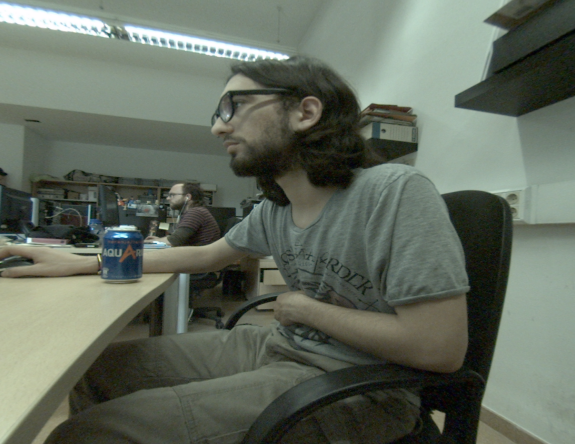
\includegraphics[width=\linewidth]{img/4}
			\caption{Original Image}
		\end{subfigure}
		\begin{subfigure}[b]{1\linewidth}
			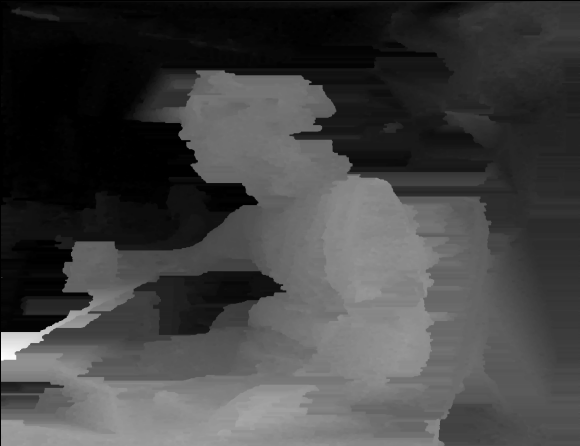
\includegraphics[width=\linewidth]{img/4b}
			\caption{Depth map image.}
		\end{subfigure}
		\caption{Original and depth map obtained using the LIBELAS library.}
		\label{fig:depthmap}
	\end{figure}
	
	\subsection{Second development phase}
	
	As its explained in the planning changes, we realized that the visualization of the streams inside the screen was not perfect and that the size of the objects was not customizable. To achieve a better experience, the screen paradigm was change, instead of displaying an image at full resolution and move it around the QT scene, a ROI of the image was selected and placed in a fixed position inside the QT scene. In this version rather than moving the image, the ROI over the image is the element that moves. This allow the user to control better the ROI and the zoom inside the image. Leaving them without any overlap between images.  

	It is worth to mention that the development team of the hardware prototype has finished the third prototype, in Figure \ref{fig:proto}, it now has an improved holding system that ensures that the camera will not move during our tests. Previously, despite our efforts to keep the camera movements at minimum, every time we started recording after calibration, the movement of the HMD or even the tension on the wire, ended up moving, and therefore decalibrating the cameras.   
	
	Related with the task \ref{obj:dataset:record}, the viewer has been ported to a 64 bits architecture, consequently, the number of frames that can be stored in memory has grown significantly. this will allow us to record longer dataset videos.
	
	Related with the task \ref{obj:dispmap}, a color map has been added to improve the visibility of the depth. This was added  because for humans is easier to see a gradient of colors rather than a gradient of grays.  
	
	Secondly after reading some papers about stereo we arrived to the conclusion that a Siamese architecture is the best option to create our neural network. A Siamese neural network is a net composed with two completely separated input layers, in our case, one for each camera. After some layers of feature extraction, we arrive to a layer where the two separated nets converge into one layer, after this layer we have some more layers where the inputs are compared and some feature extraction and feature extraction.
	
	Taking in account that the first user testing phase has been done with a limited amount of users, we have extracted some interesting conclusions, Table \ref{tab:userTestResults}. It seems that there are two types of users, the ones that feel comfortable since the beginning of the test and do not feel the need to change the presets, and the users that need to customize the distance between images to feel comfortable.
	We notice that the users that did not change much the distance between image did not feel dizzy when using a setting in different distance than the original. On the contrary, the users that did change the distance between images mostly felt dizzy when using a setting set for a different distance than they were seeing. At the same time, we notice that in most cases, both types of users feel when using the close setting in large distances objects are seen further away, and vice versa in case of far settings in closer distances.
	Moreover, we also notice that some users found difficult to find the keys used to move the images, for that reason we decided to move the keys that change the position of the right image from i,j,k and l to the arrow keys. We also notice some other little inconveniences while doing the test, for that reason a part of the protocol will be changed to improve the experience and commodity of the users.
	
	

\begin{table}
	\begin{center}
		\begin{tabular}{ccccccc}
			\toprule
			 & \multicolumn{2}{c}{Close} & \multicolumn{2}{c}{Medium} & \multicolumn{2}{c}{Far} \\ 
			Feelings & $\Delta X$ & $\Delta Y$ & $\Delta X$ & $\Delta Y$ & $\Delta X$ & $\Delta X$ \\ 
			\midrule
			Not dizzy & 0 & 12 & 6 & 0 & -18 & 0 \\ 
			\midrule 
		 	Dizzy & 6 & 0 & -258 & 0 & -114 & 30 \\ 
			\midrule
			Not dizzy & 6 & 0 & 6 & 0 & 6 & 0 \\ 
			\midrule 
			Dizzy & 6 & -6 & -66 & 12 & -72 & -6 \\ 
			\midrule
			Dizzy & -24 & 0 & -132 & 0 & -84 & 0 \\ 
			\midrule
			Dizzy & -48 & 0 & -78 & 10 & -90 & -12 \\ 
			\bottomrule
		\end{tabular} 
	\caption{Results of the vergence in the user testing sessions. Note that $\Delta X$ means separation between the two images in the X axis and $\Delta Y$ means separation in the Y axis. }
	\label{tab:userTestResults}
	\end{center}
\end{table}
	
	

	\section{Acknowledgment}
	This work is supported in part by a CVC transfer project with ProCare Light company, and partially funded by the Spanish Ministry of Economy and Competitiveness and FEDER under grants TIN2014-56919-C3-2-R and TIN2017-89723-P.
	
	\bibliography{biblio}
	\bibliographystyle{plain}

	\appendix

	\section{Objective and tasks list}
	\begin{enumerate}
		\item \label{obj:viewer} Modular HMD Viewer 
		\begin{enumerate}
			\item Preset Shortcuts
			\item Better program configuration
			\item Better viewer scene
		\end{enumerate}
	
		\item Dataset generation
		\begin{enumerate}
			\item Calibration dataset
			\item \label{obj:dataset:record} Recording module
			\item \label{obj:dataset:video} Video dataset
		\end{enumerate}
	
		\item \label{obj:dispmap} Disparity map
		\begin{enumerate}
			\item Calibration
			\item Depth map
			\item Calibration dataset
			\item \label{obj:dispmap:eval} Depth map evaluation
		\end{enumerate}
	
		\item \label{obj:acc} Accommodation-Vergence
		\begin{enumerate}
			\item \label{obj:acc:preset} Preset creation
			\item \label{obj:acc:dispmap} Disparity map
			\item \label{obj:acc:nn} Neural network
			\item User testing
		\end{enumerate}
	
		\item Depth of field blur
		\begin{enumerate}
			\item Mock-up blur
			\item Disparity map Version
			\item Neural network Version
			\item User testing
		\end{enumerate}
	
		\item \label{obj:third} Third eye
		\begin{enumerate}
			\item Integration of the viewer
			\item Research mixture of images
		\end{enumerate}
	
		\item Screen quality
	\end{enumerate}


	\begin{landscape}
		\section{Gantt planning}
		\begin{figure}[b!]
			\centering
			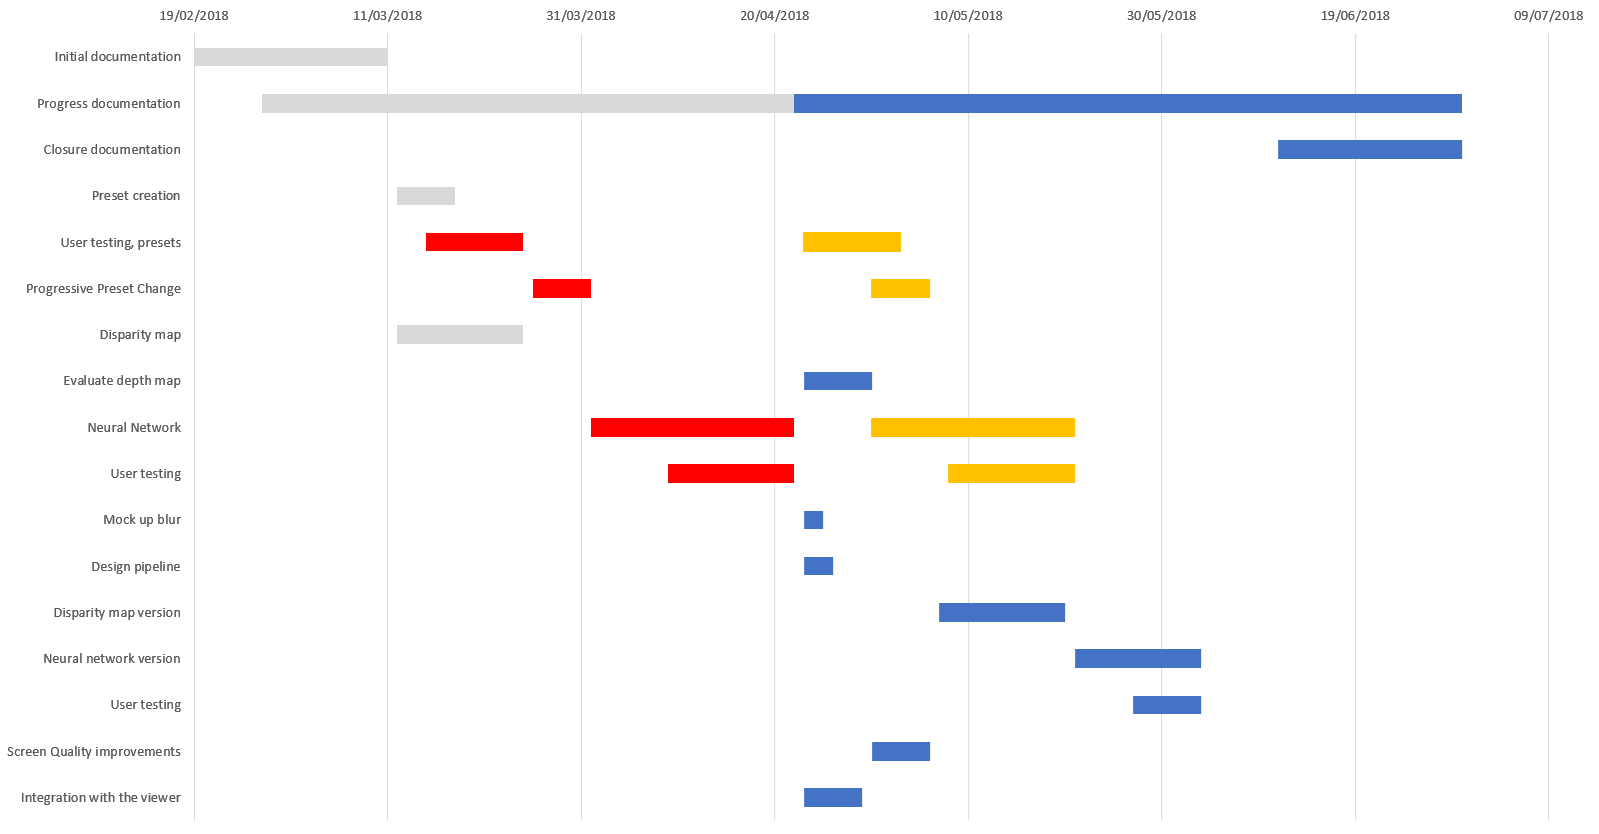
\includegraphics[width=1\linewidth]{img/gantt2}
			\caption{Gantt diagram of the project. Note that red blue tasks are remaining tasks, grey task are done tasks, red tasks are tasks not done in the scheduled time and yellow tasks are rescheduled tasks.}
			\label{fig:gantt}
		\end{figure}
		
	\end{landscape}
	
	
	
	
\end{document}

